% !TEX root = ../main.tex

\chapter{Recursion proofs}

This chapter serves as an intermediary background exploration, 
diving into more advanced concepts beyond last chapters concepts. 
The realm of zero knowledge is dynamic and continuously evolving, 
marked by ongoing advancements and active research endeavors. Among these advancements, 
recursion proofs is one of the most important and active subject. Recursion proofs are created to accelerate
 the generation of multiple zero-knowledge proofs. 
 Not all recursion proofs are created equal, they can vary significantly and serve different use cases. 
 In this section, we will examine these variations, distinguishing between them. 
 We aim to identify the most suitable method for our daily proof of liabilities and proof of inclusion.


 \cite{Nova23} for aggregation, recusrion and folding

 \section{Aggregation}
 Aggregation is the first and simples type of recursion for zk proofs. It comprises of 2 different phases.
 Initially, you create a standard individual proof for multiple blocks. In the second phase, a proof of proof is created.
 You could either merge all proofs into a single one, or do tree like structure where each parent node proove its child nodes.

This is a quite simple process. Each block as its own proof, and then you prove that the other proofs are valid, giving you only one prove 
to verify at the end. Since there is 2 different phase, 2 different circuits needs to be constructed.
On the surface, you can parallize the initial proofs, which decrease the proving time, and you only have one proof to verify, which decrease the verfying time.
However, there are still some issues with aggregation. The most important issue is that the proof time of the second circuit grows linearly with the number of blocks to verify, making it less scalable. \cite{Nova23}
 \begin{figure}[H]
    \centering
    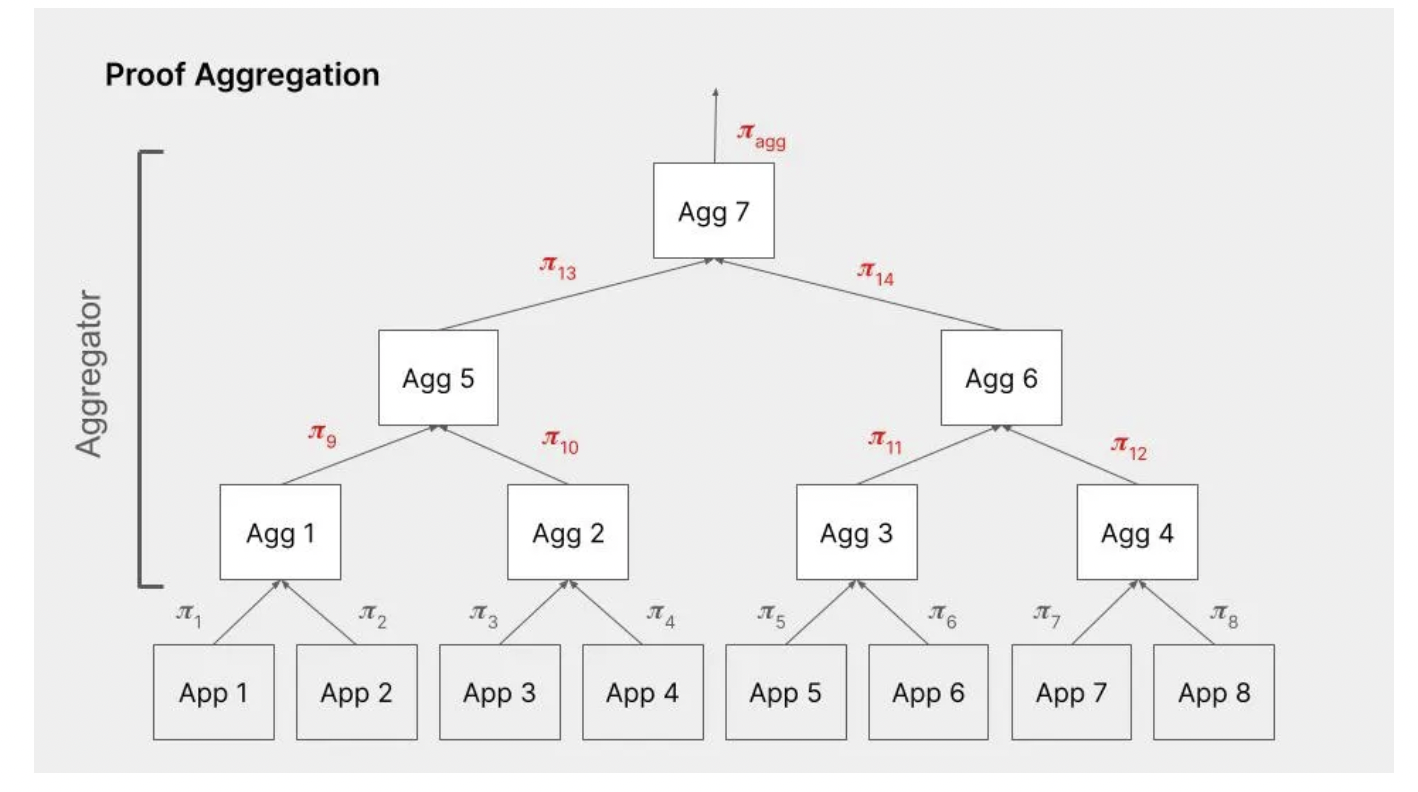
\includegraphics[width=130mm]{AggregationProof.png}
    \caption{Aggregation Proof \cite{TP24}}
    \label{overflow}
    \end{figure}

 \section{Recursion scheme} 
The next technique is the recursion scheme. Like the aggregation, the proof is separated into blocks. However, in this case each block proves that it is valid, and that the previous proof is valid. The number of constraints will always stay the same because it is only proving 2 things of fixed sizes. It is an improvement from the previous technique, but every block still has to verify the previous block, which can take some time.

\section{Accumulation}
To mitigate the exponential growth of recursion proofs, the new scheme created by nova defers every computationnaly heavy tasks to the end. 
All the defered parts are accumulate at a later point. Unlike the aggregation scheme, the last part of accumulation does not grow with every new step.
Instead of doing n times heavy work, we are doing it only once.
The heavy part of the verification step in most SNARKS is found when opening the polynomial commitment.

\subsection{Polynomial Commitments}

A polynomial commitment is a cryptographic technique that allows to commit (lock) data, and reveal (unlock) it later.

The commitments are binding, meaning there is no way to alter data once it is commited. They are also significantly shorter than
the data commited. Collisions are inevitable given the vastness of potential data sets mapped onto compact commitments (pigeonhole principle).
However, it is computationally infeasible to find a second dataset matching the same commitment.

The commimtents can also be hidden. This means that no information is shared to the receiving party. 
An example of a commitment scheme would be to hash a dataset with a collision-resistant hash function such as SHA256, and the hash value is shared.
To add the hiding property, a random string could be added at the beginning of the dataset.

Instead of commiting to a dataset, we could be commiting to a polynomial. While a commitment to the coefficient would work, we would be revealing the polynomial
when opening the commitment. We would like to be able to open the commitment only to a certain point of the polynomial. 
We are also interested in keeping the polynomial secret. An interesting property of polynomials, is that is is evaluatable at specific points.
A polynomial commitment is proving to another party that we have a commitment to a plynomial that evaluates to a certain value at a certain point.

Polynomials support linear opperations like addition or multiplication. A commitment can be additively homomorphic if the sum of the commitment values
is equal to the sum of the polynomials.

Polynomial commitments are essentials to SNARKs. Verifying opening claims of polynomial commitments constitues the computationally intensive task we mentionned earlier. \cite{VR23}


\subsection{Halo accumulation}

The concept of deferring the polynomial commitment opening checks, and consolidating them into a single operation, was introduced by Bowe, Grigg, and Hopwood Halo.\cite{BGH23}
The task of checking an opening claim for a polynomial commitment is defined in two steps.
The first part is fast, where you just output a pair of a polynomial and its commitment. The second part is expensive, where we verify the pair (f1, C1) of polynomial f1 and its commitment C1.
The second part can be accumulated if the commitment scheme is additively homomorphic. 
Instead of verifying each pair (C1 is a commitment for f1, C2 is a commitment for f2, etc.), we can verify the linear combination of every pairs (c1+c2+... is a commitment for f1+f2+...). \cite{VR23}


\section{Folding scheme} 
There is a new technique implemented by Nova, which is called the Folding Scheme. The setup is similar to the recursion scheme, but instead of computing the proof of the previous block, the R1CS are folded together at every block. Instead of having X set of R1CS, we are left with 1 set. The new R1CS are called relaxed R1CS, and are used to compute a single proof at the end of the folding.
